\chapter{Skeleton de Hamilton-Jacobi}
\label{ch:siddiqi}

La metáfora del incendio de Blum \cite{Blum:1967} dice que el \textit{skeleton} de un objeto se puede obtener encendiéndole fuego a toda su frontera simultáneamente. Luego, se asume que los frentes de llamas se propagan a una velocidad constante hacia el interior del objeto. Una vez que el fuego ha alcanzado todo el objeto, el \textit{skeleton} queda formado en los lugares donde dos frentes distintos se encontraron. En otras palabras, el \textit{skeleton} corresponde a los puntos de extinción, donde el fuego no pudo seguir avanzando por haberse encontrado consigo mismo. Estos puntos se conocen hoy en día como \textit{puntos de choque} \cite{leymarie2003three}.

Es posible simular directamente el frente de propagación de Blum como un flujo geométrico homogéneo \cite{kimmel1995skeletonization}. Sin embargo, enfrentar el problema específico de encontrar los puntos de choque (y por lo tanto, el \textit{skeleton}) permite simplificar los cálculos de varias maneras. Con ese propósito, los autores del algoritmo descrito en este capítulo recurrieron a herramientas de la mecánica lagrangiana.

\section{Fundamentos teóricos}
 
El desarrollo teórico subsecuente pertenece a la geometría diferencial. En consecuencia, la palabra \textit{objeto} ve alterado provisoriamente su significado dentro de esta sección. Los objetos 2D pasan a ser superficies cerradas y los objetos 3D pasan a ser volúmenes.

\subsection{Flujo de acortamiento de curvas}
Dado un objeto siendo atravesado por un frente de propagación, sea $\boldsymbol{C}(t)$ su frontera en el instante $t$. Es decir, $\boldsymbol{C}(t)$ es la frontera de la porción interior del objeto que en el instante $t$ todavía no ha sido alcanzada por el frente de propagación. $\boldsymbol{C}$ es una curva cerrada en 2D y una superficie cerrada en 3D. Además, $\boldsymbol{C}(0)$ es la frontera original del objeto. El movimiento del frente está dado por
\begin{equation}
\frac{\partial{\boldsymbol{C}}}{\partial{t}} = f\boldsymbol{n}
\end{equation}

\noindent
donde $f$ es la rapidez constante de propagación y $\boldsymbol{n}$ es el vector unitario normal interior a $\boldsymbol{C}$. Esta ecuación dice que, para un $\epsilon$ muy pequeño, $\boldsymbol{C}(t + \epsilon)$ se obtiene si todos los puntos de $\boldsymbol{C}(t)$ se mueven hacia el interior de $\boldsymbol{C}(t)$ con rapidez $f$ durante un tiempo $\epsilon$. En 2D es denominada \textit{flujo de acortamiento de curvas}. Su validez se sostiene para el caso 3D, donde describe la contracción de una superficie.

No existe un método analítico que sea capaz de detectar los puntos de choque directamente a partir de la ecuación (5.1), aunque sí es posible encontrarlos mediante una simulación numérica \cite{sethian1996fast}. Un enfoque más eficiente comienza por mostrar que esta ecuación en un caso particular de la \textit{ecuación de la eikonal}.

Sea $T$ un gráfico de la solución de la ecuación anterior. Es decir, $T$ es un campo escalar, donde cada paso en la evolución de $\boldsymbol{C}$ es asociado con el instante cuando ese paso tiene lugar. En otras palabras
\begin{equation}
T(\boldsymbol{C}(t)) = t.
\end{equation}

\noindent
Tomando la derivada con respecto al tiempo
\begin{equation}
\frac{d}{dt}T(\boldsymbol{C}(t)) = 1
\end{equation}
\begin{equation}
\frac{\partial T}{\partial \boldsymbol{C}}\cdot\frac{\partial \boldsymbol{C}}{\partial t} = 1
\end{equation}
\begin{equation}
\nabla T\cdot\frac{\partial \boldsymbol{C}}{\partial t} = 1.
\end{equation}

\noindent
Sustituyendo $\frac{\partial \boldsymbol{C}}{\partial t}$ usando la ecuación (5.1),
\begin{equation}
\nabla T\cdot f\boldsymbol{n} = 1
\end{equation}
\begin{equation}
||\nabla T|| f = 1.
\end{equation}

\noindent
Teniendo la ecuación (5.7) se afirma que $T$ satisface la \textit{ecuación de la eikonal}, un concepto fundamental de la óptica geométrica \cite{luneburg1964mathematical}.

A continuación se presenta una breve introducción a algunos conceptos de mecánica y óptica, necesarios para comprender la solución de esta ecuación, con los cuales el lector de computación podría no estar familiarizado. El objetivo es mostrar la relación existente entre las ecuaciones de la eikonal y la de Hamilton-Jacobi, que da nombre a este algoritmo. Las principales referencias para las siguientes subsecciones son los libros de Shankar \cite{shankar2012principles} y Arnold \cite{arnol2013mathematical}.

\subsection{Introducción a la mecánica lagrangiana}

Una partícula se encuentra en el eje horizontal $x$. Más precisamente, está posicionada sobre el punto $x_0$ en el instante $t_0$. Luego, sobre ella actúa un potencial (o fuerza) horizontal $V(x)$. Finalmente, debido a la acción de este potencial, en el instante $t_f$ se ha movido a la posición $x_f$. ¿Qué determina que su movimiento haya sido rectilíneo, a lo largo del eje $x$? ¿Por qué la partícula no escogió otro camino (por ejemplo, una curva) para llegar a $x_f$?

De acuerdo a la formulación lagrangiana, el movimiento de la partícula está restringido por el \textit{principio de mínima acción}. La \textit{acción} de cada posible camino $x(t)$ se define como
\begin{equation}
S[x(t)] = \int_{t_0}^{t_f} \! \mathcal{L}(x, \dot{x}) \, \mathrm{d}t
\end{equation}

\noindent
donde $\mathcal{L}$ es una función llamada \textit{lagrangiano}, cuyo valor es la diferencia entre las energías cinética y potencial de la partícula. El lagrangiano normalmente depende de la velocidad y la posición, que a su vez dependen del tiempo. Como es costumbre en mecánica, se usa la notación de Newton para la diferenciación: $\dot{x}$ indica la derivada de la posición con respecto al tiempo. Además, los paréntesis cuadrados se usan para indicar que $S$ es un \textit{funcional}, es decir, que depende de todo el camino $x(t)$ y no del valor de $x$ en algún instante $t$. El principio de mínima acción dice que la partícula clásica escogerá el camino $x_{cl}(t)$ que minimice $S$.

En general, como se demuestra en \cite{shankar2012principles}, el lagrangiano para el camino $x_{cl}(t)$ satisface la \textit{ecuación de Euler-Lagrange}
\begin{equation}
\frac{d}{dt} \frac{\partial\mathcal{L}}{\partial \boldsymbol{\mathrm{\dot{q}}}} - \frac{\partial\mathcal{L}}{\partial\boldsymbol{\mathrm{q}}} = 0,
\end{equation}

\noindent
donde $\boldsymbol{\mathrm{q}} = (q_1, q_2,... ,q_n)$ representa el conjunto de $n$ coordenadas independientes (o \textit{grados de libertad}) que determinan la posición de la partícula, y $\boldsymbol{\mathrm{\dot{q}}} = (\dot{q_1}, \dot{q_2},... , \dot{q_n})$ su velocidad. La ecuación (4.9) es central en mecánica, pues permite obtener las ecuaciones del movimiento simplemente derivando el lagrangiano.

La ecuación de Euler-Lagrange demuestra que las ecuaciones de la mecánica lagrangiana se sostienen para un sistema de coordenadas arbitrario. Sin embargo, en el contexto de esta tesis bastará con $\boldsymbol{\mathrm{q}} = (x, y, z)$.

\subsection{El formalismo hamiltoniano}

La mecánica hamiltoniana es una reformulación de la mecánica lagrangiana. Como se señaló anteriormente, en la mecánica lagrangiana las ecuaciones del movimiento derivan del lagrangiano $\mathcal{L}(\boldsymbol{\mathrm{q}}, \boldsymbol{\dot{\mathrm{q}}})$, el cual depende de la posición y la velocidad. En la mecánica hamiltoniana, en cambio, las ecuaciones del movimiento se obtienen a partir del \textit{hamiltoniano} $\mathcal{H}(\boldsymbol{\mathrm{q}}, \boldsymbol{\mathrm{p}})$, que depende de la posición y los \textit{momentos}. Estos últimos son cantidades que originalmente se derivan del lagrangiano:
\begin{equation}
\boldsymbol{\mathrm{p}} = \frac{\partial\mathcal{L}}{\partial\boldsymbol{\dot{\mathrm{q}}}}.
\end{equation}

\noindent
Sin embargo, la \textit{transformada de Legendre} permite transformar el lagrangiano $\mathcal{L}$ en el hamiltoniano $\mathcal{H}$ mediante la sencilla equivalencia
\begin{equation}
\mathcal{H}(\boldsymbol{\mathrm{q}}, \boldsymbol{\mathrm{p}}) = \boldsymbol{\mathrm{p}} \cdot \boldsymbol{\mathrm{\dot{q}}} - \mathcal{L}(\boldsymbol{\mathrm{q}}, \boldsymbol{\dot{\mathrm{q}}}).
\end{equation}

\noindent
Tomando la derivada parcial con respecto a $\boldsymbol{\mathrm{p}}$ se comprueba que esta transformada efectivamente invierte los roles de $\boldsymbol{\mathrm{p}}$ y $\boldsymbol{\dot{\mathrm{q}}}$: ahora la velocidad $\boldsymbol{\dot{\mathrm{q}}}$ se deriva del hamiltoniano,
\begin{equation}
\boldsymbol{\dot{\mathrm{q}}} = \frac{\partial \mathcal{H}}{\partial \boldsymbol{\mathrm{p}}}.
\end{equation}

\noindent
Además, es posible usar la ecuación (5.10) para reemplazar $\frac{\partial \mathcal{L}}{\partial \boldsymbol{\dot{\mathrm{q}}}}$ por $\boldsymbol{\mathrm{p}}$ en la ecuación (5.9). Al mismo tiempo, tomar la derivada parcial con respecto a $\boldsymbol{\mathrm{q}}$ en la ecuación (5.11) resulta en $-\frac{\partial \mathcal{L}}{\partial \boldsymbol{\mathrm{q}}} = \frac{\partial \mathcal{H}}{\partial \boldsymbol{\mathrm{q}}}$. Incorporando ambos resultados a la ecuación (5.9) se obtiene
\begin{equation}
\boldsymbol{\dot{\mathrm{p}}} = -\frac{\partial \mathcal{H}}{\partial \boldsymbol{\mathrm{q}}}.
\end{equation}

\noindent
Las ecuaciones (5.12) y (5.13) se conocen como las \textit{ecuaciones canónicas de Hamilton}. 

\subsection{}

\section{Visión general del algoritmo}

\begin{algorithm}[H]
\caption{Extracción del \textit{skeleton} de Hamilton-Jacobi}
\label{alg:hjskel}
\begin{algorithmic}[1]
\Function{SkeletonDeHamiltonJacobi}{$I$, $\tau$}
	\State $D \gets TDE(I)$
    \State $\nabla D \gets Gradiente(D)$
    \State $\mathcal{F} \gets FlujoEmergentePromedio(\nabla D)$
    \State $h \gets maxHeap()$
    \ForAll {$p$ en el borde de $I$}
    	\If {$p$ es simple}
        	\State $h.insert(p, \mathcal{F}(p))$ \Comment $p$ se inserta con el flujo como clave de ordenamiento
        \EndIf
    \EndFor
    \While {$h.size() > 0$}
    	\State $p \gets h.extractMax()$
        \If {$p$ es simple}
        	\If {$p$ no es punto de término o $\mathcal{F}(p) > \tau$}
            	\State Remover $p$ de $I$
                \ForAll {$q \in V_{26}(p)$} 
                	\If {$q$ es simple}
                    	\State $h.insert(q, \mathcal{F}(p))$
                    \EndIf
                \EndFor
            \Else
            	\State Marcar $p$ como no removible
            \EndIf
        \EndIf
    \EndWhile
    \State \Return $I$
\EndFunction
\end{algorithmic}
\end{algorithm}

\section{Detalle de la implementación}

\section{Resultados}

\begin{figure}[ht]\centering
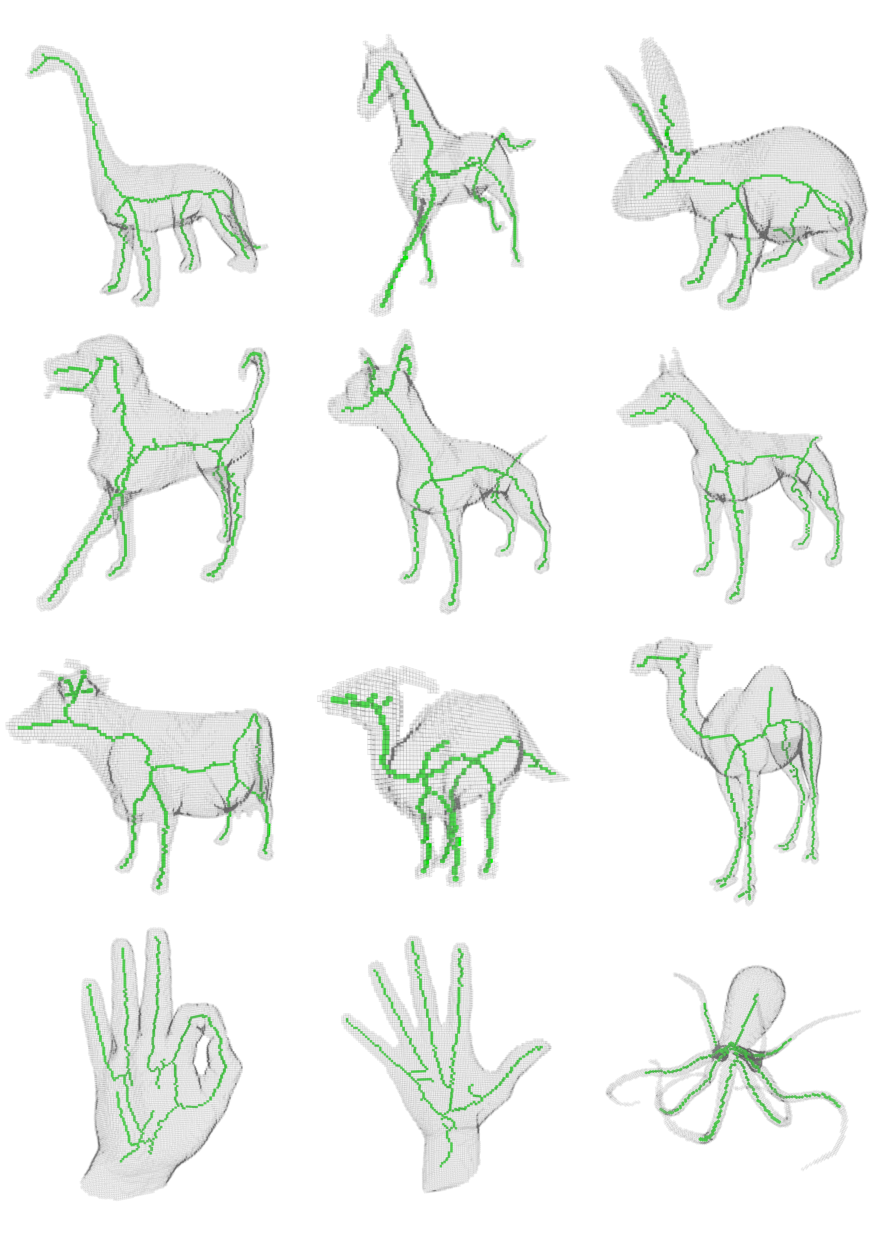
\includegraphics[width=1\linewidth]{images/siddiqi-15_test_models}
\caption{Resultados del algoritmo de Siddiqi et al. para las imágenes de prueba, con $\tau = -15$}
\label{fig:siddiqi-15_test_models}
\end{figure}

\begin{figure}[ht]\centering
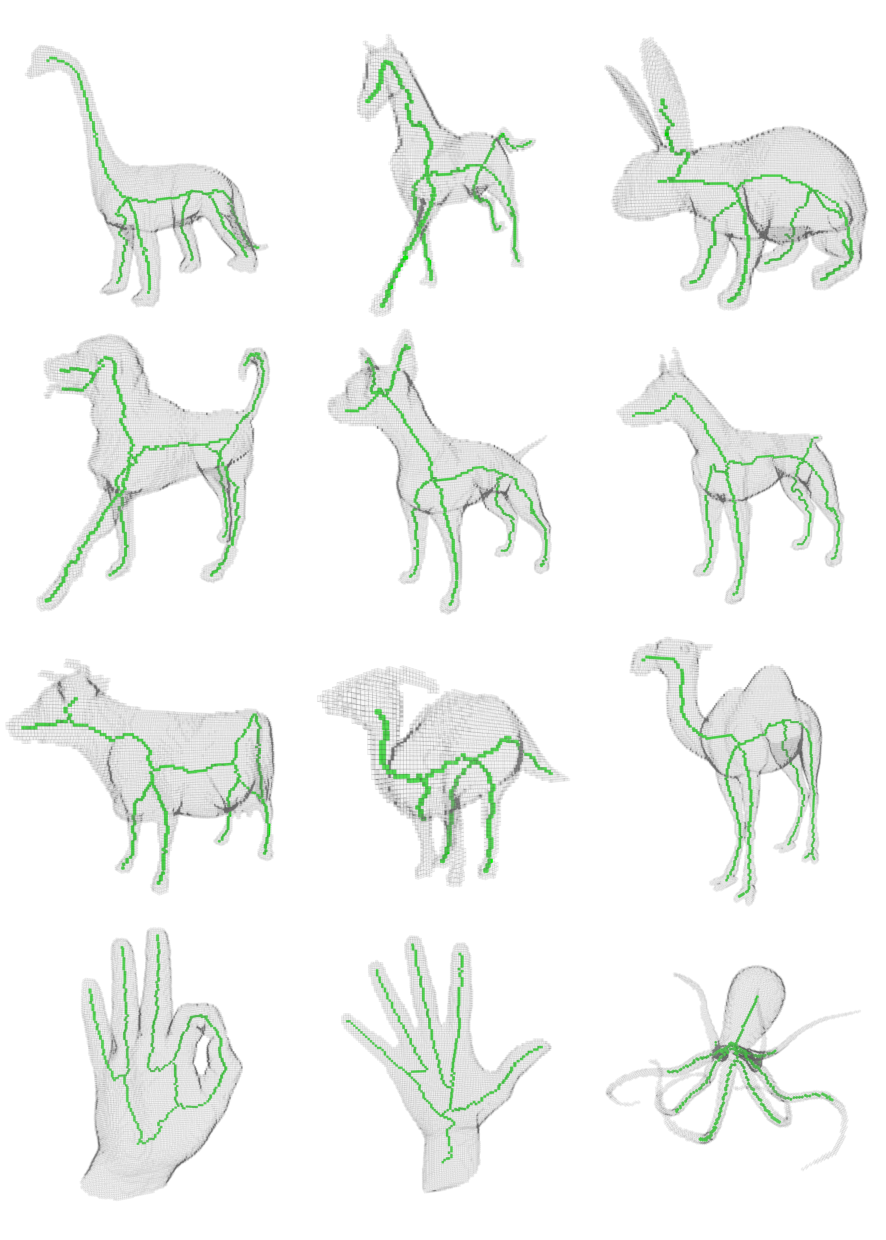
\includegraphics[width=1\linewidth]{images/siddiqi-18_test_models}
\caption{Resultados del algoritmo de Siddiqi et al. para las imágenes de prueba, con $\tau = -18$}
\label{fig:siddiqi-18_test_models}
\end{figure}